\subsection{Hadamardovy matice}
% 6 predn

\begin{definition}[Hadamardova matice (HM)]
    Hadamardova matice čádu $m$ je $H\in\{-1,1\}^{m\times m}$ taková, že $HH^T=mI_m$.
    $m$ na diagonále znamená, že všechny souřadnice jsou nenulové.
    Nuly mimo diagonále - řádky jsou ortogonální.
\end{definition}
\begin{lemma}[Transpozice Hadamardovy matice]
    $H$ je Hadamardova matice, právě když $H^T$ je Hadamardova matice.
\end{lemma}
\begin{proof}
	Kvůli symetrii pojmů, stačí jedna implikace směrem.
	Podělíme matici $\sqrt{m}$:
	\[ \left(\frac{1}{\sqrt{m}} H \right) \left(\frac{1}{\sqrt{m}} H^T \right) = I \]
	Neboli
	\[ \left(\frac{1}{\sqrt{m}} H \right) = \left(\frac{1}{\sqrt{m}} H^T \right)^{-1} = \sqrt{m}H^{-1} \]
	Tedy
	\[ H^T H = m H^{-1}H = mI \]
\end{proof}

\begin{definition}[Normální forma HM]
	Hadamardova matice je v \emph{normální formě}, pokud všechny prvky v prvním řádku a prvním sloupci jsou +1.
\end{definition}

\begin{observation}[Uzavřenost HM]\label{hm_close}
	Přehození řádků či sloupců, stejně tak jako vynásobení řádku či sloupce $-1$, zachovává vlastnost "býti Hadamardovou maticí".
	Každou HM lze tedy vynásobením vhodných řádků a sloupců číslem $-1$ převést na HM stejného řádu, která je v normálním tvaru.
\end{observation}

\begin{theorem}[Hadamardova matice a řád dělitelný čtyřmi]\label{hm_4}
    Je-li $m>2$ řád HM, pak $m\equiv 0\mod 4$.
\end{theorem}
\begin{proof}
	Triviální případy: $m = 1$ matice je skalár.
	Pro $m = 2$ máme jedinou možnost
	\[ H = \begin{pmatrix} 1 & 1\\ 1 & -1 \end{pmatrix} \]

	Nechť $H$ je HM v normální formě, $m > 2$.
	Řádkovými a sloupcovými úpravy převedeme matici na následující tvar
	\[ H = \begin{pmatrix}
		a & b & c & d \\
		||| & ||| & ||| & ||| \\
		||| & ||| & --- & --- \\
		||| & --- & ||| & --- \\
            	\vdots  & \vdots  & \ddots & \vdots
	      \end{pmatrix}
	\]

	Uvažme prvky v prvních třech řádcích. V prvním řádku jsou všechny prvky $+1$.
	Budiž $a$ počet sloupců, ve kterých má jak druhý, tak třetí řádek $+1$, $b$ počet sloupců, ve kterých má druhý řádek $+1$ a třetí řádek $-1$, $c$
	počet sloupců, ve kterých má druhý řádek $-1$ a třetí řádek $+1$, a konečně $d$ počet sloupců, ve kterých má jak druhý, tak třetí řádek $-1$.
	Z ortogonality řádků vyplývá, že
	\begin{gather*}
		a + b + c + d = m\\
		a + b - c - d = 0\\
		a - b + c - d = 0\\
		a - b - c + d = 0
	\end{gather*}
	Sečtením 2 a 3 rovnice dostaneme $a = d$.
	Sečtením 1 a 4 rovnice $a = d = \frac{m}{4}$.
	Pak 1 a 2 dostaneme $b = \frac{m}{4}$.
	Neboli soustava má jediné řešení $a = b = c = d = \frac{m}{4} \Rightarrow m \equiv 0 \mod4$.
\end{proof}

\begin{theorem}[Hadamardova matice a symetrické BIBDy]
    HM řádu $m=4t$ existuje $\iff$ existuje symetrický $(4t-1,2t-1,t-1)$-BIBD.
\end{theorem}
\begin{proof}
	Nechť $H$ je HM v normální formě.
	Vyškrtneme první řádek a sloupec, čímž dostaneme matici velikosti $(4t - 1)$.
	Tak nahradíme $-1 \to 0$.
	Nechť matice po úpravách je $A$.

	Z vlastnosti HM, matice $A$ má v každém sloupci $(2t - 1)$ jedniček.
	Ekvivalentně:
	\[ JA = (2t - 1) J \]
	Neboli $A$ jako matice incidence množinového systému implikuje, že každá množina má $(2t - 1)$ prvků.
	Zkontrolujeme ještě, že 2 prvky leží ve stejném počtu bloků $\to$ skalární součin 2 řádků.
	Pro 2 libovolné řádky (kromě prvního) platí, že mají na čtvrtině míst $(t - 1)$ $1$ proti $-1$, viz důkaz \cref{hm_4}.

	Transformace matice lze provést i opačným směrem, což dává ekvivalenci.
\end{proof}

\begin{definition}[Tenzorový součin]\label{tenzs}
	Jsou-li $A\in T^{m\times m}, B\in T^{n\times n}$, indexujeme prvky $A$ jako $a_{ij}$, pak jejich tenzorový součin je matice (bloková):
    \[
        A\times B=\begin{pmatrix}
            a_{11}B & a_{12}B & \ldots & a_{1m}B\\
            a_{21}B & a_{22}B & \ldots & a_{2m}B\\
            \vdots  & \vdots  & \ddots & \vdots\\
        \end{pmatrix}
    \]
\end{definition}

\begin{theorem}[Kombinace Hadamardových matic]\label{hm_komb}
    Existují-li HM řádů $m_1,m_2$, pak existuje HM řádu $m_1\cdot m_2$.
\end{theorem}
\begin{proof}
	Nechť výsledná matice je $H$.
	Dostaneme ji pomoci tenzorového součinu \cref{tenzs} daných matic.
	Z konstrukce, každý blok nové matice dostaneme násobením HM $H_2$ prvkem $a_{ij} \in \{ -1, 1 \}$.
	Dle \cref{hm_close} $H \in \{ 0, 1 \}^{m_1 \cdot m_2 \times m_1 \cdot m_2}$.

	Vezmeme 2 libovolné řádky $H$ ze stejného bloku, jejich skalární součin je
	\[ \sum_{j = 1}^{n_1} a_{ij}^2 \langle H_2, H_2 \rangle = \sum_{j = 1}^{n_1} a_{ij}^2 \cdot 0 \]
	Pro 2 řádky z různých bloků (pro $u \ne w$ dopadne stejné jako předchozí):
	\[ u = w: \sum_{j = 1}^{n_1} a_{ij} \cdot a_{kj} \langle H_2, H_2 \rangle = \sum_{j = 1}^{n_1} a_{ij}^2 \cdot m_2 \]
	Vytkneme $m_2$ ze sumy a dostaneme skalární součin $i$-ho a $j$-ho řádku matice $H_1$, což je taky nula.
\end{proof}

\begin{consequence}[Sylvester]\label{sylv_cons}
	HM řádu $2^k$ existuji pro $\forall k \in \N$.
\end{consequence}

\begin{conj}[Hadamard]
	HM řádu $m$ existuje pro každé $m = 4t$.
\end{conj}

\begin{consequence}[Exponenciální Hadamardovy matice]
    Pro každé $k$ existuje HM řádu $2^k$.
\end{consequence}
\begin{theorem}[Payleyho konstrukce]
    \begin{itemize}
        \item[a)] Je-li $q=p^r$ mocnina prvočísla $p$ a $q\equiv 3\mod 4$, pak existuje HM řádu $q+1$.
        \item[b)] Je-li $q=p^r$ mocnina prvočísla $p$ a $q\equiv 1\mod 4$, pak existuje HM řádu $2q+2$.
    \end{itemize}
    Případ pro $q = 2$ je pokrytý kvůli \cref{sylv_cons}.
\end{theorem}
\begin{proof}
	Vezměme konečné těleso $GF(q)$.
	Definujme \emph{kvadratický charakter} $\chi:GF(q) \to \{ -1, 0, 1 \}$:
	\[ \chi(x) = \threepartdef{0}{x = 0}{1}{\exists y \in GF(q): x = y^2}{-1}{jinak} \]
	Znovu $\square$-zbytky a nezbytky.
	Jelikož multiplikativní grupa je cyklická s generátorem $g$, pak $\square$-zbytek je $g^{2k}$ a nezbytky naopak liché mocniny.
	Proto
	\[ \chi (xy) = \chi(x) \cdot \chi(y) \]
	Taky máme polovinu $\square$-zbytků a polovinu nezbytků, tak
	\begin{equation}\label{chi_all}
		\sum_{b \in GF(q)} \chi(b) = 0
	\end{equation}

	Z čehož odvodíme:
	\begin{lemma}[Posunutí $\chi$]\label{chi_lemma}
		\[ \forall c \ne 0: S = \sum_{b \in GF(q)} \chi(b) \chi(b + c)= -1 \]
	\end{lemma}
	\begin{proof}
		Vyjádříme $(b + c)$ jako $b \cdot y$.
		\[ y = \frac{b + c}{b} \]
		pro $b = 0$ charakter je nula, takové sčítanci neovlivňuji součet, proto
		\[ S = \sum_{b \ne 0 \in GF(q)} \chi(b) \chi(b + c) \]
		Taky nahlédneme, že $y$ je jednoznačné a zobrazení $b \to y$ je prosté a na $\Rightarrow$ bijekce.
		Navíc $b = \frac{c}{y - 1}$ platí vždy protože pro $y = 1$ bychom dostali $c = 0$.
		\[ S = \sum_{b \ne 0} \chi(b) \chi(by)= \sum_{y \ne 1} \chi(b)^2 \chi(y) \stackrel{\chi^2(b) = 1}{=} \sum_{y \ne 1} \chi(y) = \sum \chi(y) - \chi(1) = -1 \]
	\end{proof}

	\begin{definition}[Charakterová matice Q]\label{char_q}
		Označme $GF(q) = \{ a_1, \ldots, a_q \}$, definujme matici $Q \in \{ -1, 0, 1 \}^{q \times q}$ předpisem
		\[ Q_{ij} = \chi(a_i - a_j) \]
	\end{definition}

	Nechť $\bar{1}$ je vektor délky $q$, $\forall i: \bar{1}_i = +1$

	a) pokud $q\equiv 3\mod 4$, pak
	\[ H_{q + 1} = \begin{pmatrix} 0 & \bar{1} \\ -\bar{1}^T & Q \end{pmatrix} + I_{q + 1} \]
	je HM řadu $(q + 1)$.
	Dostaneme matici
	\[ H = \begin{pmatrix}
		| & | & | & | & | & \ldots \\
		- & | & q & q & q & \ldots \\
		- & q & | & q & q & \ldots\\
		- & q & q & | & q & \ldots \\
		\vdots & \vdots & \vdots & \vdots & \ddots & \vdots
	      \end{pmatrix}
	\]
	Z definici $Q$ a vlastnosti konečného tělesa $Q$ má mimo diagonálu $-1 \lor 1$.
	Neboli $H \in \{ -1, 1 \}^{q + 1 \times q + 1}$.
	Skalární součin řádku se sebou, $i > 0$:
	\[ S = -1 + 1 + \sum_{j = 1}^q \chi(a_i - a_j) \]
	Jelikož $j \in [q]$, tak suma probíhá všemi prvky $GF(q)$, dle \eqref{chi_all} je 0.
	Takže $S = 0$.

	Skalární součin dvou libovolných řádků, $i, k > 0$:
	\[ S = 1 + \chi(a_k - a_i) + \chi(a_i - a_k) + \sum_{j = 1}^q \chi(a_i - a_j) \chi(a_k - a_j) \]
	Pak
	\[ \chi(a_k - a_i) + \chi(a_i - a_k) = \chi(a_k - a_i) + \chi(-1(a_k - a_i)) = \chi(a_k - a_i) + \chi(-1)\chi(a_k - a_i)) \stackrel{\chi(-1) = -1}{=} 0 \]
	Kde $q \equiv 3 \mod 4 \Rightarrow \chi(-1) = -1$.
	Použijeme \cref{chi_lemma} na
	\[ \sum_{j = 1}^q \chi(a_i - a_j) \chi(a_k - a_j) \]
	tak, že $b = a_i - a_j$ a $c = a_k - a_i \ne 0$.
	Neboli součet je $-1$.

	Dokázali jsme taky
	\[ QJ = 0 = JQ \]
	A
	\[ QQ^T = \begin{pmatrix} q - 1 & -1 \\ -1 & \ddots \end{pmatrix} = qI_q - J \]

	b) Pokud $q\equiv 1\mod 4$, sestavíme HM řádu $2q+2$ takto:
	\[ H_{2q + 2} = \begin{pmatrix}
		0 & \bar{1} & 0 & \bar{1} \\
		\bar{1}^T & Q & \bar{1}^T & Q \\
		0 & \bar{1} & 0 &- \bar{1} \\
		\bar{1}^T & Q & -\bar{1}^T & -Q \\
	      \end{pmatrix}
	+ \begin{pmatrix} I_{q + 1} & -I_{q + 1}\\ -I_{q + 1} & -I_{q + 1} \end{pmatrix}
	\]
	Technickým rozborem případů ověříme, že $H_{2q + 2}$ je HM.
\end{proof}

\begin{lemma}[O tenzorovém součinu (BD)]\label{tzs_lemma}
    Pro $A,A_1,A_2$ čtvercové matice řádu $m$, $B,B_1,B_2$ čtvercové matice řádu $n$:
    \begin{itemize}
        \item $(A\times B)^T=A^T\times B^T$
        \item $\forall \alpha\in T: \alpha(A\times B)=(\alpha A)\times B=A\times(\alpha B)$
        \item $(A_1+A_2)\times B=A_1\times B+A_2\times B$
        \item $A\times(B_1+B_2)=A\times B_1+A\times B_2$
        \item $(A_1\times B_1)(A_2\times B_2)=(A_1A_2)\times(B_1B_2)$
    \end{itemize}
\end{lemma}
%\begin{proof}
%    TODO; technický
%\end{proof}

\begin{observation}[Tenzorový produkt I]
	\[ \forall m,n: I_m \times I_n = I_{mn} \]
\end{observation}

\begin{theorem}[Kombinace HM alternativní]\label{hm_komb_a}
    Existují-li HM řádů $m_1,m_2$, pak existuje HM řádu $m_1\cdot m_2$.
\end{theorem}
\begin{proof}[Alternativní důkaz věty o kombinaci Hadamardových matic]
	Nechť $A$ je HM řadu $m_1$, $B$ řadu $m_2$.
	Pak z \cref{tzs_lemma}
	\[ (A \times B)(A \times)^T = (A \times B)(A^T \times B^T) = (AA^T)\times (BB^T) = (mI_m)\times (nI_n) = mn I_{mn} \]
\end{proof}

\begin{note}[Tenzorový součin symetrických matic]
	Pokud jsou matice A, B symetrické, je i jejich tenzorový součin symetrická matice.
	Takže pokud existují symetrické HM řádů $m_1$ a $m_2$, pak existuje symetrická HM řádu $m_1 m_2$.
\end{note}

\begin{theorem}[Payleyho konstrukce revisited]
\end{theorem}
\begin{proof}
	a) Nechť $Q$ je matice definovaná jako \cref{char_q}, pak označme
	\begin{equation}\label{will_s}
		S = S_{q + 1} = \begin{pmatrix} 0 & \bar{1} \\ -\bar{1}^T & Q \end{pmatrix}
	\end{equation}
	Pak platí:
	\begin{gather*}
		QJ = 0 = JQ \\
		QQ^T = qI_q - J \\
		SS^T = q I_{q + 1}
	\end{gather*}

	Z $q \equiv 3 \mod 4 \Rightarrow \chi(-1) = -1$, matice $S$ je \emph{antisymetrická}: $S^T = -S$ proto pro $H_{q + 1} = S + I_{q + 1}$ platí:
	\[ H_{q + 1} H_{q + 1}^T = (S + I_{q + 1})(S^T + I_{q + 1}) = SS^T + S^T + S + I_{q + 1} = qI_{q + 1} - S + S + I_{q + 1} = (q + 1) I_{q + 1} \]
	Neboli dle definice $H_{q + 1}$ je HM.

	b) je speciální případ tzv Williamsonové konstrukce kterou ukážeme níže.
\end{proof}

\begin{lemma}[Williamson]\label{will_lemma}
    Buď $S\in\R^{n\times n}$ t.ž.
    \[ SS^T=(n-1)I_n \& S^T=\varepsilon S, \varepsilon\in \{-1,1\} \]
    Mějme $A,B\in\R^{m\times m}$ takové, že
    \[ AA^T=BB^T=mI_m, AB^T=-\varepsilon BA^T \]
    Pak pro matici
    \[ K=A\times I_n + B\times S \]
    platí $KK^T=mnI_{mn}$.
\end{lemma}
\begin{proof}
	\begin{gather*}
		KK^T = (A \times I_n + B \times S)(A^T \times I_n + B^T \times S^T) = \\
		= AA^T \times I_n + AB^T \times S^T + BA^T \times S + BB^T \times SS^T = \\
		= m I_m \times I_n + (-\varepsilon BA^T) \times (\varepsilon S) + BA^T \times S + m I_m \times (n - 1)  I_n \\
		= m I_{mn} + (-\varepsilon^2 + 1)(BA^T \times S) + m(n - 1) I_{mn} \stackrel{(-\varepsilon^2 + 1) = 0}{=} mn I_{mn}
	\end{gather*}
\end{proof}
\begin{theorem}[Williamsonova konstrukce]
    Buď $q=p^r$ mocnina prvočísla $p$ a $q\equiv 1\mod 4$ a existuje HM řádu $h>1$.
    Potom existuje HM řádu $h(q+1)$.
\end{theorem}
\begin{proof}
	Pro matici $S$ definovanou v \eqref{will_s} platí:
	\[ S^T = S \& SS^T = q I_{q + 1} \]
	protože $q \equiv 1 \mod4$ je $-1 \square$-nezbytek. Nebol $S$ splňuje předpoklady \cref{will_lemma} pro $\varepsilon = 1$.

	Nechť $A$ je HM řádu $h$.
	Sestrojíme pomocnou $U$:
	\[ U = I_{\frac{h}{2}} \times \begin{pmatrix} 0 & 1 \\ -1 & 1 \end{pmatrix} \]
	Což je komplikovaný zápis pro matici, která má 0 na hlavní diagonále.
	Na dvou vedlejších diagonálách se střídá $1, -1$.
	Položme
	\[ B = UA \]
	Pak
	\begin{gather*}
		BB^T = UAA^TU^T = U(hI_h)U^T = hUU^T = hI_H(= AA^T), \\
		AB^T = AA^TU^T = (hI_h)U^T = -hU\\
		BA^T = UAA^T = U(hI_h) = hU
	\end{gather*}
	Neboli $S, A, B$ splňují předpoklady Williamsonova lemmatu \cref{will_lemma}.
	Proto pro
	\[ K = A \times I_{q + 1} + B \times S \]
	platí $KK^T = h(q + 1)I_{h(q + 1)}$ což je definice HM řadu $h(q + 1)$.
	Musíme ale ověřit, že prvky v $K$ jsou $\in \{ -1, 1 \}$.

	Matice $A \times I_{q + 1}$ se skládá z bloků diagonálních matic s $1$ nebo $-1$ na diagonále.
	Matice $B$ umísti do bloků buď $S$ nebo $-S$.
	Jelikož matice $Q$ má nuly na diagonále a ${-1, 1}$ mimo diagonálu v součtu na každé pozice dostaneme $0 \pm 1 = \pm 1$.

	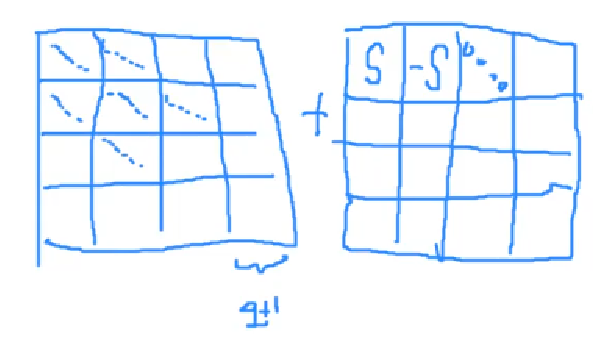
\includegraphics[scale=0.5]{will_0.eps}
\end{proof}

HW: pro jakou matici $A$ dostaneme Payleyho konstrukce z Williamsonové?
